%!TEX root = /Users/stevenmartell/Documents/CONSULTING/HumpbackChub/HBC_2011_Assessment/WRITEUP/HBCmain.tex

\section{Work plan}
The following outlines a work plan for the assessment of abundance for humpback chub. The objective is to develop a much more flexible length-based model that can be used to explore alternative hypotheses about natural mortality rates, cumulative effects of release mortality for intensive sampling periods, and to potentially integrate other sources of environmental variations such as the effects of turbidity on capture probability and recruitment variation.

\section*{Analytical approach}
I will develop a statistical catch-at-length model in the AD Model Builder software and additions R-scripts for manipulating data and summarizing model results.  Input data for the model will consist of a matrix of the total catch-at-length in 5 to 10 mm size intervals for all years, a matrix of the number of marks released by size and year, a matrix of the number of marks recaptured by size and year, and a three dimensional array of the number of marks recaptures by size for each tag-cohort released (optional).

Estimated parameter will include: natural mortality rate, growth parameters, a vector of the initial numbers in each length interval, and a vector of age-0 recruits each year.  Propagation of the numbers-at-length to the next time step will be based on a size-transition matrix, which is a function of the growth parameters and variation in growth.  Observation models will include a probability of capturing an animal of a given length each year, the probabilities of capturing a marked and unmarked animal of a given length, and optionally the probability of recapturing a specific tag-cohort of a given length.  These predicted observations will be compared with the empirical data using a negative binomial likelihood function.  The negative binomial model is more suitable here because it can account for over-dispersed data  and accommodate zero observations in cases where there is sparse information.

\section*{Detailed work plan}

\subsection*{Major components of the project}
The following is list of milestones for this project.  Each of these items will be expanded upon in the section on project details.
\begin{enumerate}
	\item Data acquisition and processing.
	\item Development of an operating model for simulating data with known parameter values.
	\item Development of a length-based assessment model to be fitted to data on capture and recapture information by length interval.
	\item Simulation testing; exploring the precision and bias of the assessment model in jointly estimating recruitment, size-specific capture probability, and growth and natural mortality using simulated data sets.
	\item Application of the length-based model to the HBC data.
	\item Quantifying uncertainty in model parameters and estimates of recruits using Markov Chain Monte Carlo methods to integrate the joint posterior distribution.
	\item Report \& presentation to the Technical Working Group.
\end{enumerate}

\subsection*{Project details}
\begin{description}
	\item[Data acuisition \& processing] The necessary data required to conduct the analysis will require information from the following fields in the GCMRC database: FISHNO, TRIP\_ID, DATES, RM, RIV, TL, TAGNO. The following SQL statement was used in a previous study to extract the necessary information. Note that the following code has been modified to obtain all fish lengths, not just those greater than 150 mm.
	\begin{verbatim}
		--****
		--All
		--****

		CREATE OR REPLACE VIEW FISH.V_ASMR_2009_ALL
		(
		    FISHNO,
		    TRIP_ID,
		    DATES,
		    RM,
		    RIV,
		    TL,
		    TAGNO
		)
		AS
		SELECT "CAPTURE_ID" fishno, "TRIP_ID" trip_id, "START_DATE" dates,"START_RM" rm,"RIVER_CODE" riv, "TOTAL_LENGTH" tl,"TH_ENCOUNTER_RANKING" tagno
		      FROM FISH.CAPTURE_HISTORY_20091211_0832
		     WHERE SPECIES_CODE = 'HBC'
		     AND (
		       (RIVER_CODE = 'COR' AND START_RM >= 57 AND START_RM <= 68.5)
		       OR RIVER_CODE = 'LCR'
		       )
		     AND START_DATE >= TO_DATE('04/01/1989', 'MM/DD/YYYY')
		     AND TOTAL_LENGTH >= 00
		
	\end{verbatim} 
	
	An R-script will be developed for post processing of the data to assign the length capture and recapture information into discrete length intervals for assembling input data into the assessment model.
	
	\item[Operating model] An individual based model will be developed to generate simulated data sets with known natural mortality rates, recruitment vectors, growth rates and capture probabilities.  The pseudo code for the operating model is as follows:
	\begin{enumerate}
		\item Specify a vector of absolute recruitment from 1950-2011.
		\item For each individual recruit in each year apply the following procedure:
		\begin{enumerate}
			\item boolean trail for survival, if the animal survives then go to (b) else, individual died and restart at step 2.
			\item boolean trail for capture:
			\begin{enumerate}
				\item Captured: obtain length of fish, if greater than 150mm then tag and release fish, go.
				\item Recaptured: obtain length of fish, goto step (a).
				\item Not captured: goto step (a).
			\end{enumerate}
		\end{enumerate}
		\item Store information about individual capture history and length into simulated database.
	\end{enumerate}
	The above algorithm is intended to generate the exact data that is currently collected in the HBC monitoring program. Specific details about factors that affect capture probability and survival would be incorporated into the boolean probabilities defined in 2a and 2b.
	
	\item[Length-based assessment model] A statistical length-based assessment model is similar in nature to a statistical catch-age model in that numbers-at-age, or in this case, numbers-at-length are propagated forward in time.  The previous Age-Structured Mark-Recapture Model (ASMR) was dependent on catch-age information; age data for HBC were inferred from an analytical age-length key (i.e., based on inferences about growth, not empirical age-length data).  Estimates of uncertainty were overly precise due to the pre-processing of the data to be used with ASMR. The length-based model makes no such inferences about the age of individual fish and is based strictly on the length observation data.  
	
	In a length based model, individuals in a given length interval are propagated in time by redistributing these individuals into new length bins based on a length transition probability (Fig \ref{fig:lengthTransition}).  The length transition probability is a function of growth and the time interval between sampling events.  The graphical example in Fig \ref{fig:lengthTransition} does not account for mortality over time, its only meant to show the transition of individuals from one length bin to subsequent length bins.
	\begin{figure}[htbp]
		\centering
			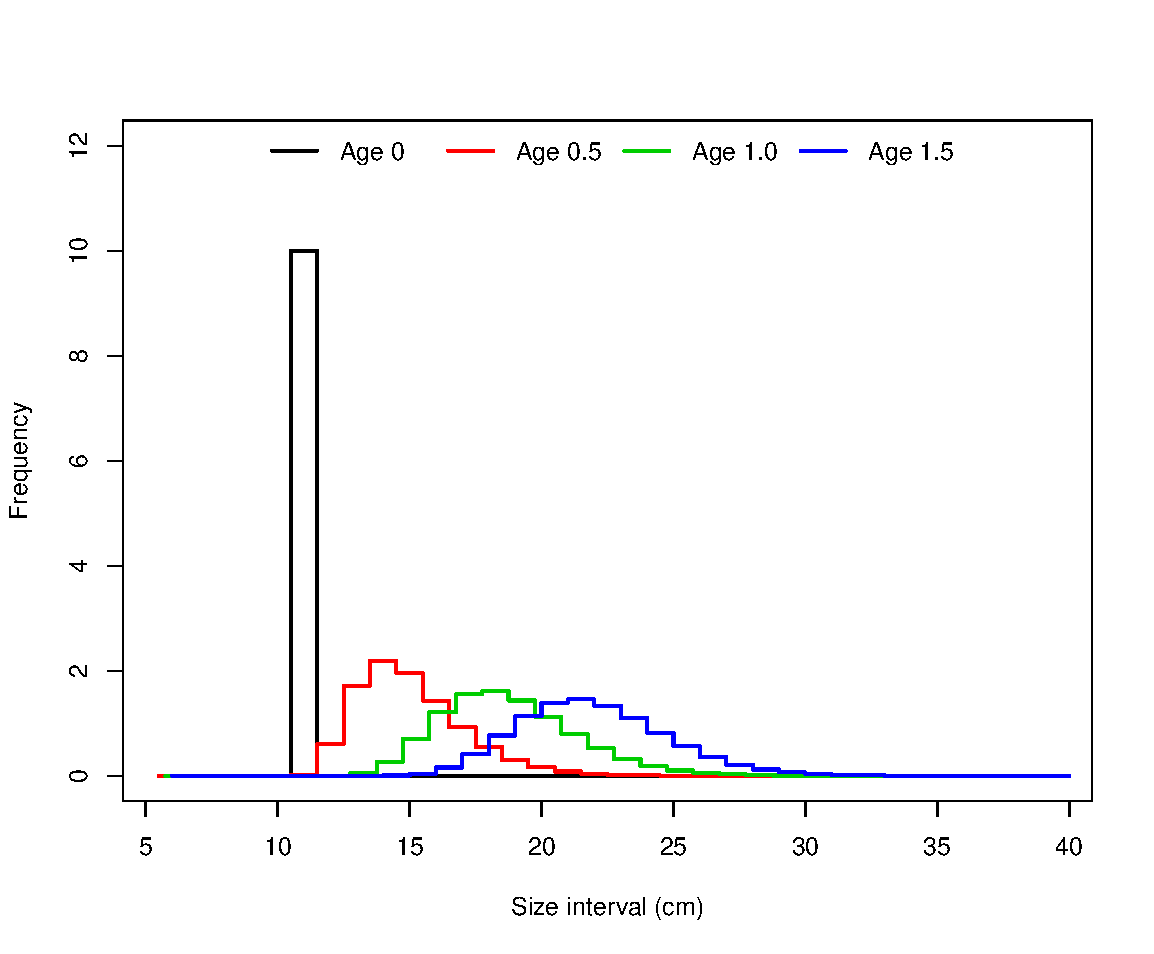
\includegraphics[scale=0.65]{../FIGS/fig:lengthTransition}
		\caption{A graphical example of a length-based transition. Starting with 10 age-0 individuals, these 10 would then be distributed to the age-0.5 distribution distribution.  The age-0.5 distribution then transitions to the age-1.0 distribution and so on.}
		\label{fig:lengthTransition}
	\end{figure}
	
	\item[Simulation testing] The purpose of simulation testing is to (i) demonstrate that the model is able to estimate the model parameters given perfect information and satisfying all of the model assumptions, (ii) examine precision and bias in parameter estimates when faced with observation, process, and structural errors, and lastly (iii) to examine the estimability, bias, and precision of model parameters when underlying structural assumptions are not met.  Simulation testing will be conducted to examine the ability to jointly estimate recruitment, capture probability, growth and natural mortality in a reliable and unbiased manner.
	
	\item[Application to the HBC data] The length-based assessment model will then be applied to the length-based capture and recapture data for the humpback chub monitoring program.  Model outputs will include estimates of recruits (and associated uncertainty), estimated model parameters (and uncertainty).  It is  anticipated that more reliable estimates of recruits will be available with the length based model because the model is not limited to length information that is greater than 150mm, as is the case in the ASMR model.
	
	\item[Quantifying uncertainty] Estimates of uncertainty will jointly consider uncertainty in the mark-recapture data, growth and mortality.  To do so the joint posterior distribution of the data will be constructed numerically using a Markov Chain Monte Carlo procedure (using the Metropolis Hastings algorithm implemented in AD Model Builder).  Uncertainty in model parameters as well as outputs will be cast in the form of marginal posterior densities.
	
	\item[Report and presentation] This is original research and the methods outlined for a length-based model that incorporates growth increment data from a mark recapture program has not been previously published to my knowledge. Ideally these results will be disseminated in the primary literature, but will also be presented to the Technical Working Group and be available as a technical report (e.g., USGS Open File Report).  Also source code, scripts, and documentation will be hosted on an open source repository with version control.  The intention here is to create a repository for continued development of the software and to document the historical changes over time.
\end{description}
